\documentclass[tikz,border=6pt]{standalone}
\usepackage{amsmath,amssymb}
\usepackage{xcolor}
\definecolor{accent}{HTML}{A13D2C}
\definecolor{accent2}{HTML}{2B5F6B}
\definecolor{muted}{HTML}{5A564F}
\definecolor{linecol}{HTML}{D8D2C4}
\definecolor{astroblue}{HTML}{1B4F72}
\usetikzlibrary{arrows.meta}
\IfFileExists{results/ch13/wd_MR.dat}{\def\datadir{results/ch13/}}{\def\datadir{../results/ch13/}}
\begin{document}
% Ideal neutron gas: TOV (solid) and Newtonian equilibrium (dashed) with the same exact Fermi pressure.
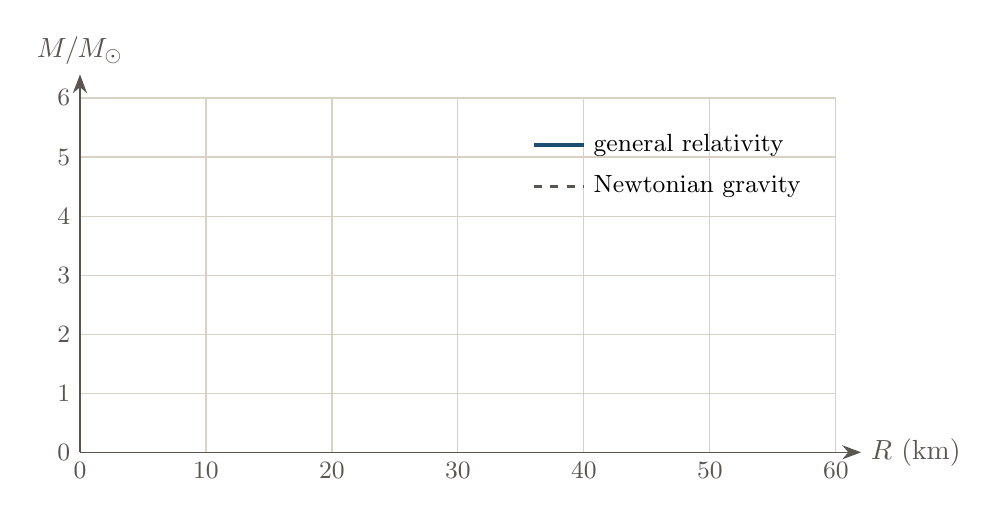
\begin{tikzpicture}[x=0.16cm,y=0.75cm, >={Stealth[length=2.4mm]}]
  \begin{scope}
    \clip (0,0) rectangle (60,6);
    \draw[linecol] (0,0) grid[xstep=10,ystep=1] (60,6);
    \draw[muted, dashed, line width=1.1pt] plot file {\datadir ns_MR_newton.dat};
    \draw[astroblue, line width=1.3pt] plot file {\datadir ns_MR_tov.dat};
  \end{scope}
  \draw[->, muted] (0,0) -- (62,0) node[right] {$R\ (\mathrm{km})$};
  \draw[->, muted] (0,0) -- (0,6.4) node[above] {$M/M_\odot$};
  \foreach \x in {0,10,20,30,40,50,60} \node[below, muted] at (\x,0) {\small \x};
  \foreach \y in {0,1,2,3,4,5,6} \node[left, muted] at (0,\y) {\small \y};
  \draw[astroblue, line width=1.3pt] (36,5.2) -- (40,5.2); \node[right] at (40,5.2) {\small general relativity};
  \draw[muted, dashed, line width=1.1pt] (36,4.5) -- (40,4.5); \node[right] at (40,4.5) {\small Newtonian gravity};
\end{tikzpicture}
\end{document}
